%!TEX TS-program = xelatex 
%!TEX encoding = UTF-8 Unicode 

\documentclass[fontsize=11pt, paper=a4, 
DIV15,
normalheadings,
parskip=half-, 
pointlessnumbers]{scrartcl}

\usepackage[british]{babel} 

\usepackage{fontspec,xltxtra,xunicode} 
\defaultfontfeatures{Mapping=tex-text} 

\setromanfont[Mapping=tex-text]{DejaVu Serif}
\setsansfont[Scale=MatchLowercase,Mapping=tex-text]{Helvetica} 
\setmonofont[Scale=1.0]{Courier New} 

\frenchspacing

\usepackage{graphicx}
\graphicspath{{../../Bilder/}}

\usepackage{longtable}

\usepackage{philokalia}

%%%

\input{../../abbreviations/abbreviations_1}

\begin{document}

\begin{center}
{\fontspec{Helvetica}{\LARGE \textbf{
Special Instructions for Text Flows
\\[3mm]
(Addendum to Data Entry Specs 2.0) 
}}} \\[5mm]
\large Wolfgang Schmidle, Klaus Thoden, Malcolm D. Hyman

\normalsize Max Planck Institute for the History of Science, Berlin, Germany

\today
\end{center}

%\tableofcontents

\section{Text Flows Within a Page}

\begin{mainrule}
Text flows are marked by §<tf>§ and §</tf>§. The text flow in italics has the number 1, i.e. §<tf 1>§, and the other text flow has the number 2, i.e. §<tf 2>§.
%Text flows are marked by §<tf>§ and §</tf>§. The text flow in Latin has the number 1, i.e. §<tf 1>§, and the text flow in Italian has the number 2, i.e. §<tf 2>§.
\end{mainrule}

\begin{clarification}
Type the §<tf>§ and §</tf>§ tags on separate lines. On each page, type the first text flow before the second text flow.
\end{clarification}

\vspace{3mm}
\begin{sampleImage}[1: \, two real pages]{conimbricenses_final_ds706707_white15}

\notTranscribed
\end{sampleImage}

\begin{note}
Both text flows have separate catchwords, which should not be typed. Each text flow may have its own marginal notes and footnotes; type them according to the rules in section 2.6.1 and 2.6.2 in the main Data Entry Specs. 
\end{note}

%\begin{sampleImage}[2: \, how to type text flows]{textflows_words2}
%\begin{sampleImage}[2: \, how to type text flows]{two_textflows.pdf}

\begin{example}[2: \, how to type text flows]

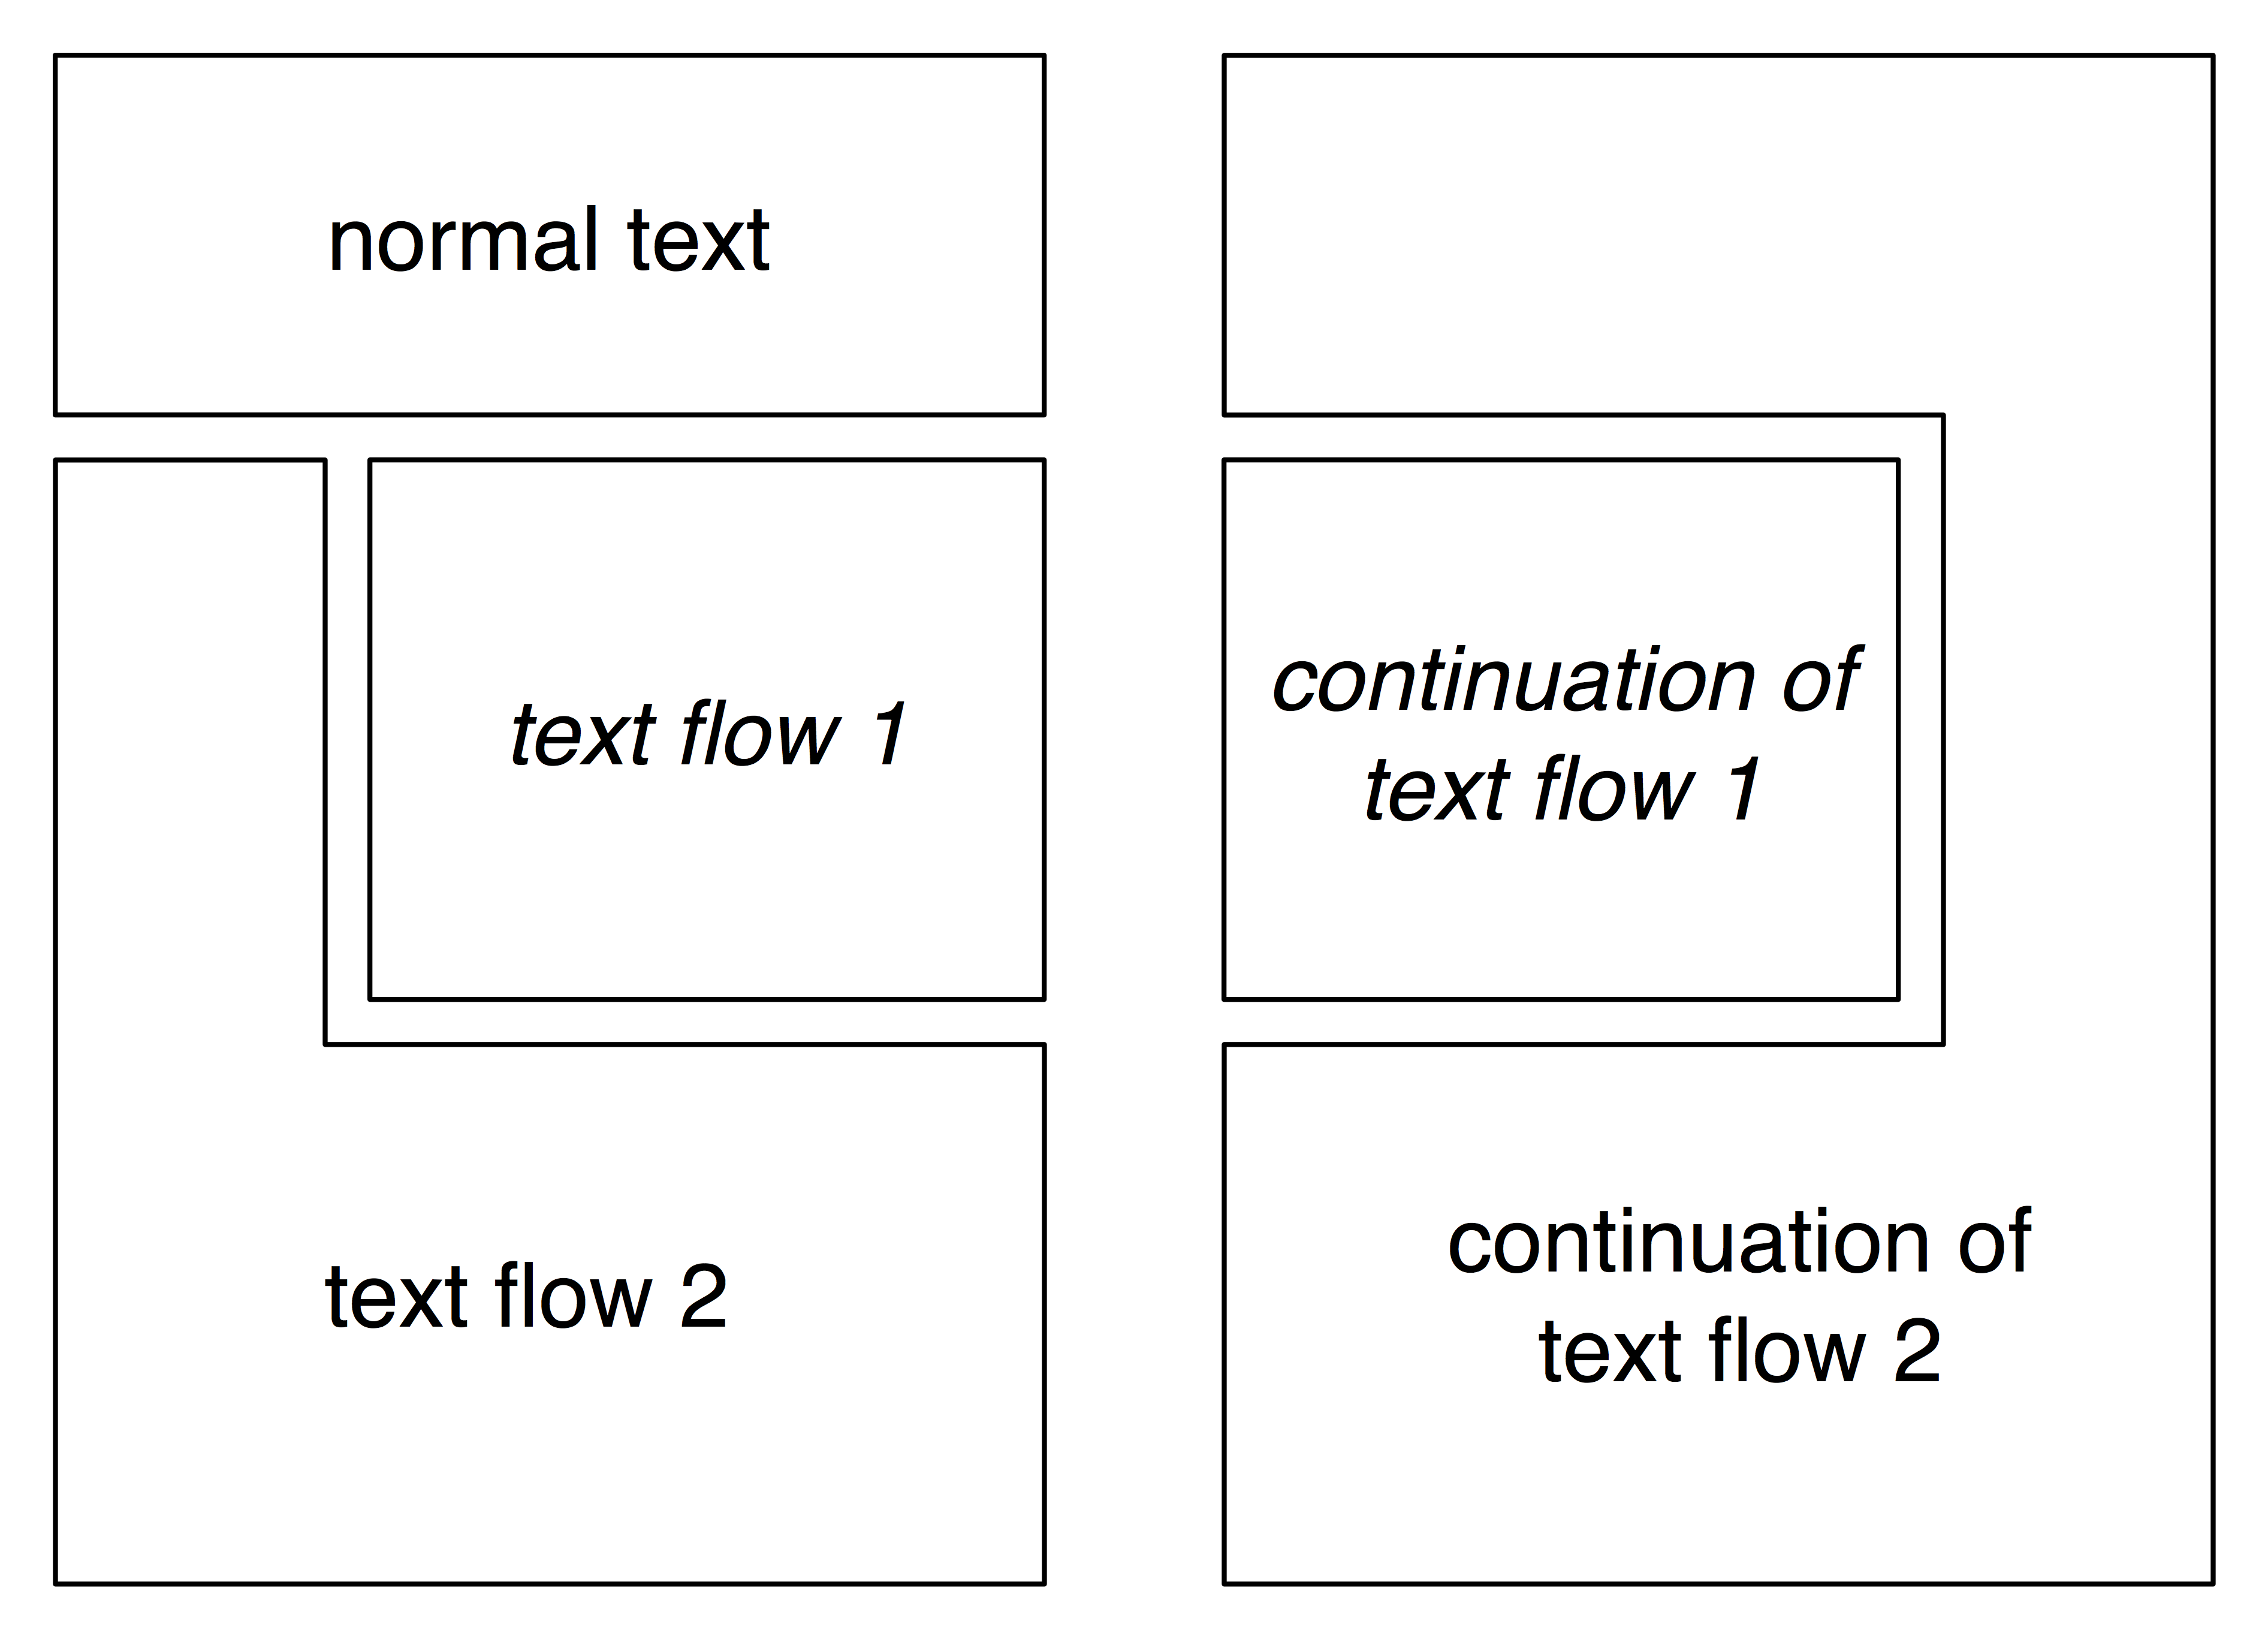
\includegraphics[width=12cm]{two_textflows.pdf}

\begin{typeLatin}
\bold{<pb>} \\
normal text \\
\bold{<tf 1 it>} \\
text flow 1 \\
\bold{</tf>} \\
\bold{<tf 2>} \\
text flow 2 \\
\bold{</tf>} \\ \\
\bold{<pb>} \\
\bold{<tf 1 it>} \\
continuation of \\ 
text flow 1 \\
\bold{</tf>} \\
\bold{<tf 2>} \\
continuation of \\ 
text flow 2 \\
\bold{</tf>} \\
\end{typeLatin}
\end{example}


%\section{Text Flows on Separate Pages}
\section{Text Flows in Vitruvius (1758)}

\begin{mainrule}
In Vitruvius (1758), please treat the pages starting from 0046.jpg up to 0489.jpg as two separate text flows, i.e. tag the main text on even pages as §<tf 1>§ and the main text on odd pages as §<tf 2>§. Do not mark the columns in the footnotes.
\end{mainrule}

\newpage
\begin{example}[3: \, text flows on separate pages]

\includegraphics[width=\linewidth]{textflow_vitruv1758_text}

\begin{typeLatin}
\bold{<pb} 268\bold{><rh>} ... \bold{</rh>} \\
\bold{<tf 1>} \\
text with some anchors\bold{<n} 1\bold{>}, a heading and some marginal notes \\
... \\
\bold{</tf>} \\ 
\bold{<fn} (a)\bold{>}footnote\bold{</fn>} \bold{<fn} (b)\bold{>}footnote\bold{</fn>} \bold{<fn} (c)\bold{>}footnote\bold{</fn>} \\
\bold{<fn} (1)\bold{>} footnote ... \bold{</fn>} \\
\bold{<fn} (2)\bold{>} footnote ... \bold{</fn>} \\
\bold{<fn} (3)\bold{>} footnote ... \bold{</fn>} \\
\\
\bold{<pb} 269\bold{><rh>} ... \bold{</rh>} \\
\bold{<tf 2>} \\
text with the same anchors\bold{<n} 1\bold{>}, heading and marginal notes \\
... \\
\bold{</tf>} \\ 
\bold{<fn>} ... footnote (3) continued\bold{</fn>} \\
\bold{<fn} (4)\bold{>} footnote ... \bold{</fn>} \\
\bold{<fn} (5)\bold{>} footnote ... \bold{</fn>} \\
\end{typeLatin}
\end{example}

%\\
%\bold{<pb>} \\
%... \\

\end{document}
